% J13: GNN predicts the active constraints of a bilevel scheduling problem
% Shared preamble for the graphical abstracts (homepage "Latest journal articles").
% Build: bash _tikz/papers/build.sh  (writes images/papers/Jxx.svg)
% Classic TikZ look: white background, black text and arrows, standard xcolor
% colors for the elements (independent of the website theme).
\documentclass[tikz,border=0pt]{standalone}
\usepackage[T1]{fontenc}
\usepackage{textcomp}
\usepackage[scaled=0.95]{helvet}
\renewcommand\familydefault{\sfdefault}
\usetikzlibrary{arrows.meta,calc,positioning,patterns,decorations.pathreplacing}
% ---- classic colors (xcolor names) ----
\colorlet{main}{blue!70!black}   % primary elements
\colorlet{lite}{blue!35}         % connections
\colorlet{pale}{blue!8}          % light fills
\colorlet{acc}{red!75!black}     % highlights / outputs
\colorlet{good}{green!55!black}  % storage, positive
\colorlet{warn}{orange!85!black} % uncertain
\colorlet{sun}{orange}
\colorlet{rule}{black!35}
\colorlet{ink}{black}
\colorlet{muted}{black!60}
\colorlet{bg}{white}
\tikzset{
  every picture/.style={line cap=round, line join=round},
  head/.style={font=\fontsize{8.5}{10}\selectfont\bfseries, text=ink},
  sub/.style={font=\fontsize{6.6}{8}\selectfont, text=muted},
  lab/.style={font=\fontsize{7.2}{8.6}\selectfont, text=ink},
  flow/.style={-{Stealth[length=2.2mm,width=2mm]}, draw=black, line width=0.9pt},
  card/.style={draw=black!60, line width=0.6pt, fill=white, rounded corners=1mm},
  banner/.style={draw=black, line width=0.6pt, fill=black!4, text=black,
                 font=\fontsize{7.4}{9}\selectfont\bfseries\boldmath, inner sep=1.6mm},
}
% canvas 8 x 6 cm (4:3), white
\newcommand\canvas{\fill[bg] (0,0) rectangle (8,6);}

\begin{document}
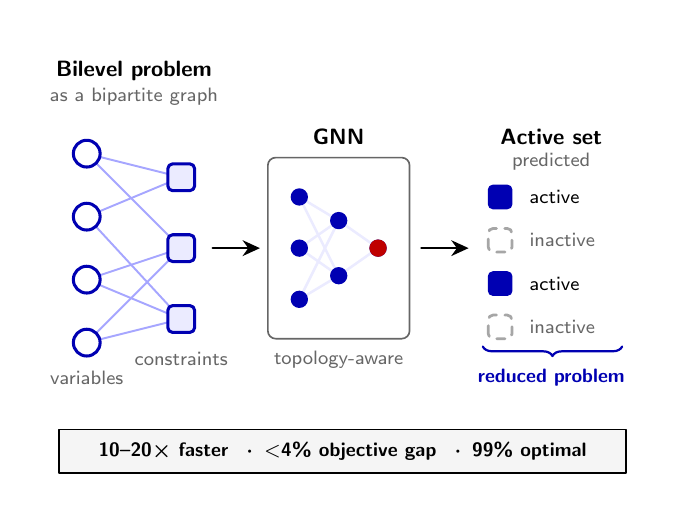
\begin{tikzpicture}
\canvas
% 1. bipartite graph
\node[head] at (1.35,5.45) {Bilevel problem};
\node[sub]  at (1.35,5.12) {as a bipartite graph};
\foreach \v/\y in {a/4.4,b/3.6,c/2.8,d/2.0} \coordinate (v\v) at (0.75,\y);
\foreach \c/\y in {x/4.1,y/3.2,z/2.3} \coordinate (c\c) at (1.95,\y);
\foreach \p/\q in {a/x,a/y,b/x,b/z,c/y,c/z,d/y,d/z} \draw[lite, line width=0.7pt] (v\p) -- (c\q);
\foreach \v in {a,b,c,d} \filldraw[fill=white, draw=main, line width=1.1pt] (v\v) circle (0.17);
\foreach \c in {x,y,z} \filldraw[fill=pale, draw=main, line width=1.1pt, rounded corners=0.6mm]
   ($(c\c)+(-0.17,-0.17)$) rectangle ++(0.34,0.34);
\node[sub] at (0.75,1.55) {variables};
\node[sub] at (1.95,1.80) {constraints};
\draw[flow] (2.35,3.2) -- (2.95,3.2);
% 2. GNN
\node[head] at (3.95,4.62) {GNN};
\draw[card] (3.05,2.05) rectangle (4.85,4.35);
\foreach \i/\y in {1/3.85,2/3.2,3/2.55} \coordinate (l\i) at (3.45,\y);
\foreach \i/\y in {1/3.55,2/2.85} \coordinate (m\i) at (3.95,\y);
\coordinate (o) at (4.45,3.2);
\foreach \i in {1,2,3} \foreach \j in {1,2} \draw[pale, line width=0.9pt] (l\i) -- (m\j);
\foreach \j in {1,2} \draw[pale, line width=0.9pt] (m\j) -- (o);
\foreach \p in {l1,l2,l3,m1,m2,o} \fill[main] (\p) circle (0.11);
\fill[acc] (o) circle (0.11);
\node[sub] at (3.95,1.78) {topology-aware};
\draw[flow] (5.0,3.2) -- (5.6,3.2);
% 3. predicted active set
\node[head] at (6.65,4.62) {Active set};
\node[sub]  at (6.65,4.30) {predicted};
\foreach \y/\s in {3.85/1,3.30/0,2.75/1,2.20/0} {
  \ifnum\s=1
    \filldraw[fill=main, draw=main, rounded corners=0.6mm] (5.85,\y-0.15) rectangle ++(0.3,0.3);
    \node[lab, anchor=west] at (6.25,\y) {active};
  \else
    \draw[rule, line width=1pt, dashed, rounded corners=0.6mm] (5.85,\y-0.15) rectangle ++(0.3,0.3);
    \node[sub, anchor=west] at (6.25,\y) {inactive};
  \fi}
\draw[main, line width=0.8pt, decorate, decoration={brace, amplitude=1.2mm, mirror}]
   (5.78,1.95) -- (7.55,1.95);
\node[lab, text=main] at (6.65,1.55) {\textbf{reduced problem}};
% result
\node[banner, minimum width=7.2cm] at (4,0.62)
   {10--20$\times$ faster \enspace$\cdot$\enspace \textless4\% objective gap \enspace$\cdot$\enspace 99\% optimal};
\end{tikzpicture}
\end{document}
